\documentclass[12pt,aspectratio=169]{beamer}
\usefonttheme[onlymath]{serif}
\usepackage{thaispec}
\usepackage{graphicx}
\usepackage{colortbl}
\usepackage{tikz}
\usepackage{xcolor}

\usetheme{Copenhagen}
\usecolortheme{crane}

\begin{document}

\title{การประมาณค่าดัชนีคุณภาพอากาศ ณ \\จุดที่ไม่มีสถานีวัด \\ (Better Estimation of Absent Air Quality Indices) } 
\date{อาจารย์ที่ปรึกษา: ดร.รัฐพรหม พรหมคำ}
\author{นางสาวหฤทัย ชาหอม รหัสนักศึกษา 116210901007-1 \\
นางสาวเบญจมาศ สินแก้ว รหัสนักศึกษา 116210901010-5 \\ 
นายกิตติคุณ ปริญญาประเสริฐ รหัสนักศึกษา 116210901021-2}

\maketitle

\begin{frame}
    \frametitle{Problem}
    \begin{tikzpicture}[overlay, remember picture]
        \node at (7,-0.8) {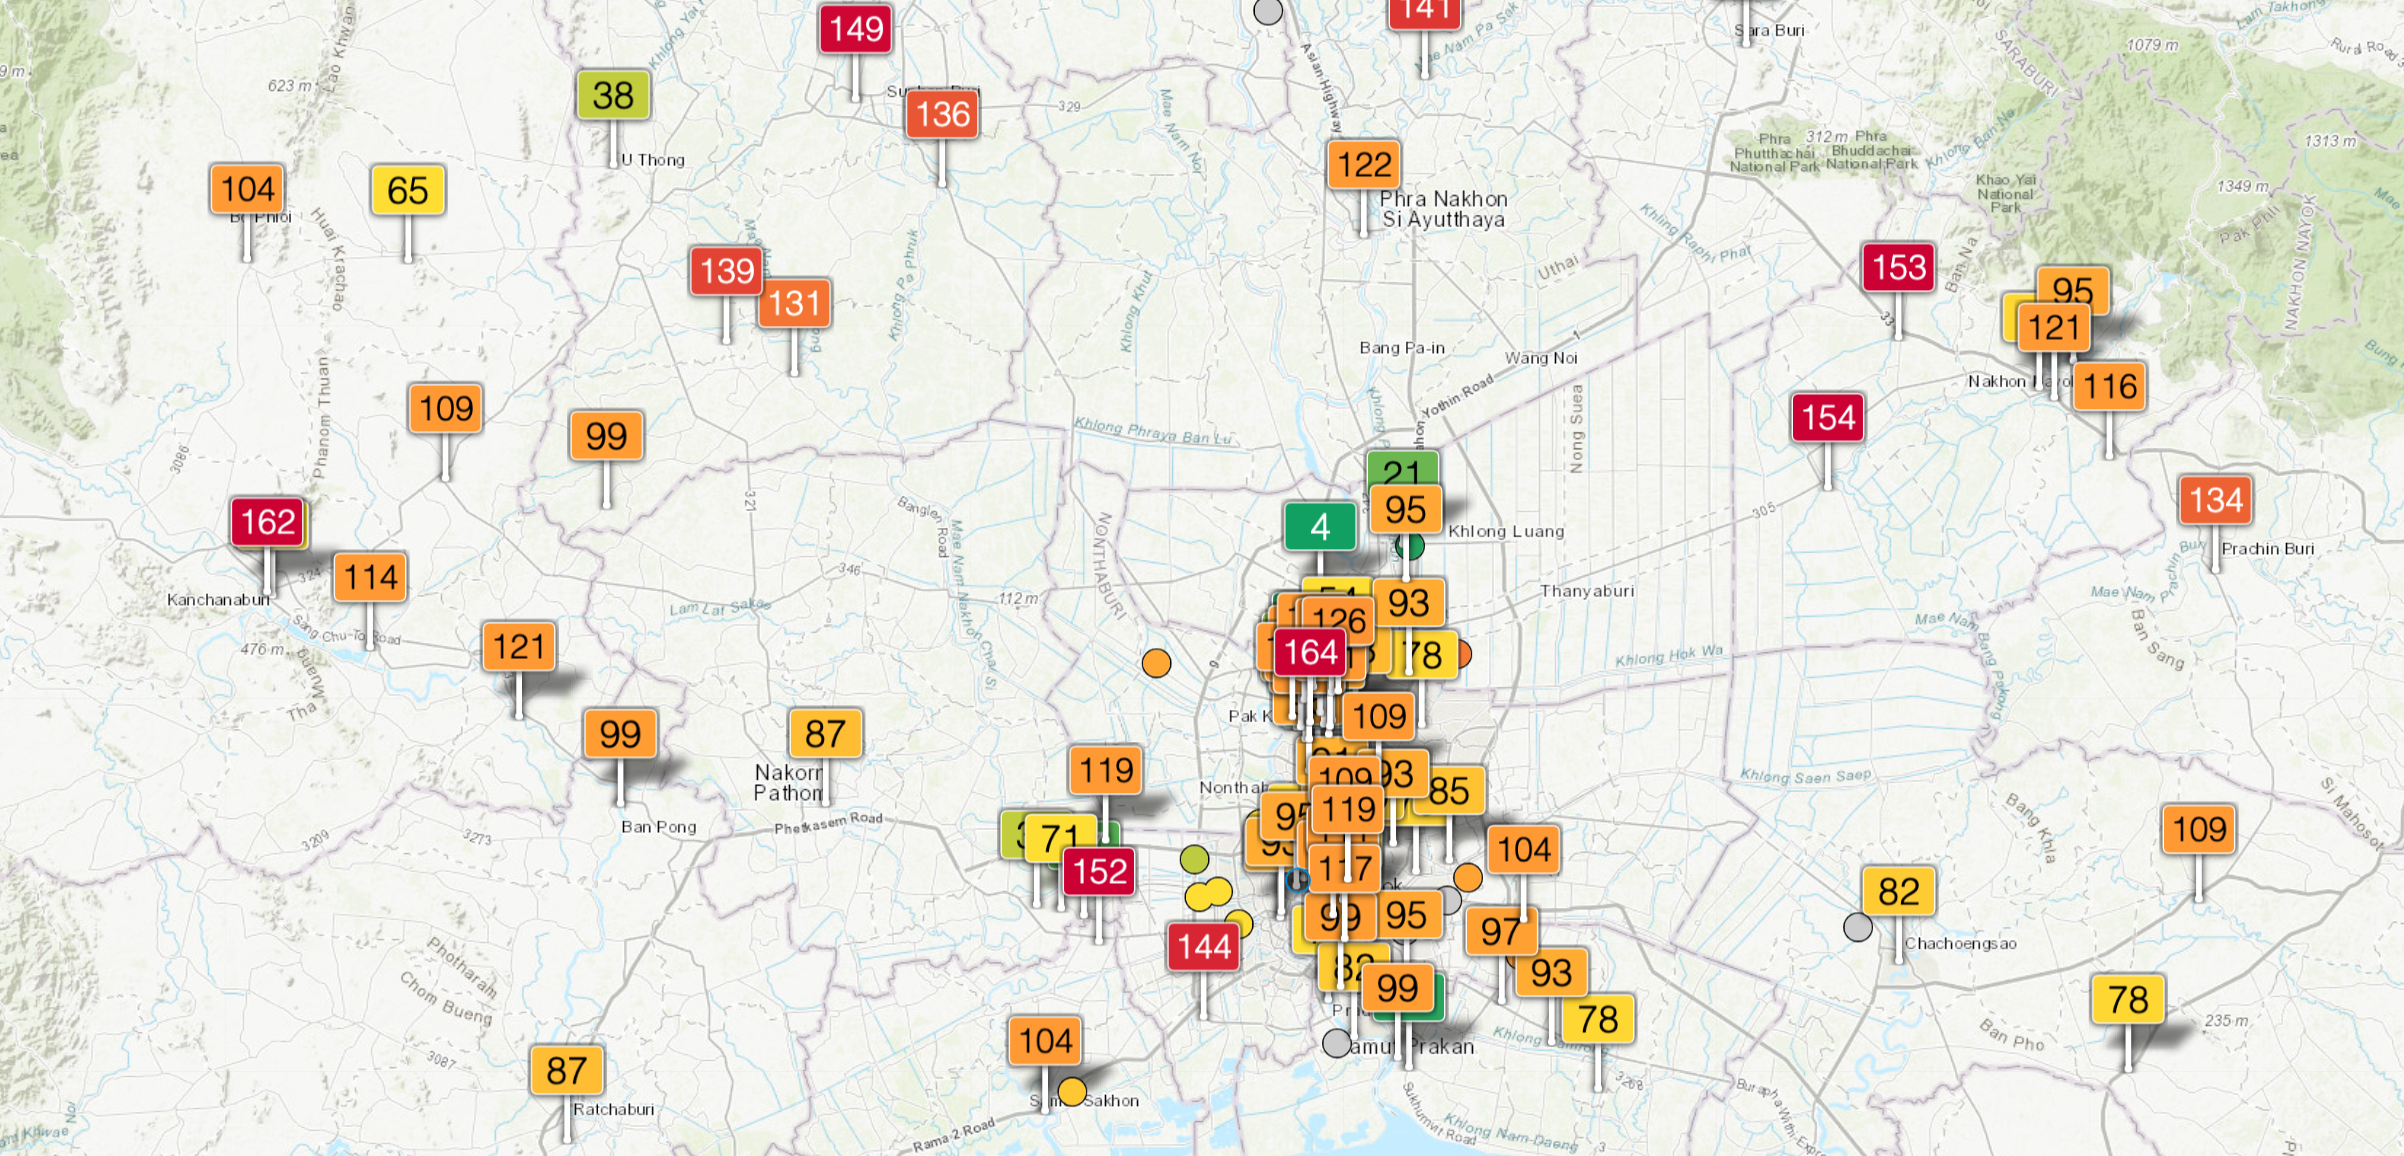
\includegraphics[width=1.25\textwidth]{img/missing-station-aqi.png}};
    \end{tikzpicture}
    \end{frame}

    \begin{frame}
        \frametitle{การประมาณค่าเชิงเส้นคู่แบบทางเลือก}
        \begin{columns}
            \begin{column}{0.5\textwidth}
            กำหนดให้ $f(x,y)$ คือ ค่า AQI ที่พิกัด $(x,y)$:
            \begin{block}{}
              \[
                    f(x,y)=a+bx+cy+dxy
               \]   
            \end{block}

               \begin{center}
                   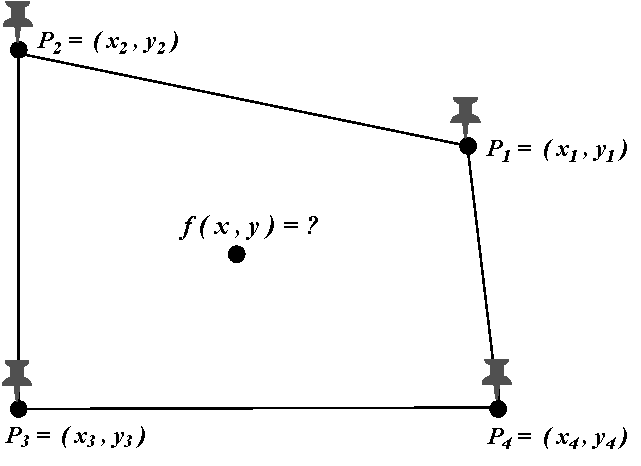
\includegraphics[width=\textwidth]{img/region-selection-one-point.pdf}
               \end{center}
            \end{column}
            \begin{column}{0.4\textwidth}  
            เมื่อ $a,b,c$ และ $d$ คือผลเฉลยของสมการ $AX = B$  โดยที่              
            \[
               A
               =\begin{bmatrix}
               1 & x_1 & y_1 & x_1y_1\\
               1 & x_2 & y_2 & x_2y_2\\
               1 & x_3 & y_3 & x_3y_3\\
               1 & x_4 & y_4 & x_4y_4\\
               \end{bmatrix},
        \]
        \[
               X = \begin{bmatrix}
                  a \\ b \\ c \\ d
               \end{bmatrix}
               ,
               B
               =\begin{bmatrix}
                  f(x_1,y_1) \\
                  f(x_2,y_2) \\
                  f(x_3,y_3) \\
                  f(x_4,y_4)
               \end{bmatrix}
        \]
            \end{column}
            \end{columns}
\end{frame}
    
\begin{frame}
\frametitle{การเเบ่งกั้นบริเวณรอบจุดเป้าหมาย}
\begin{center}
                \begin{figure}
                    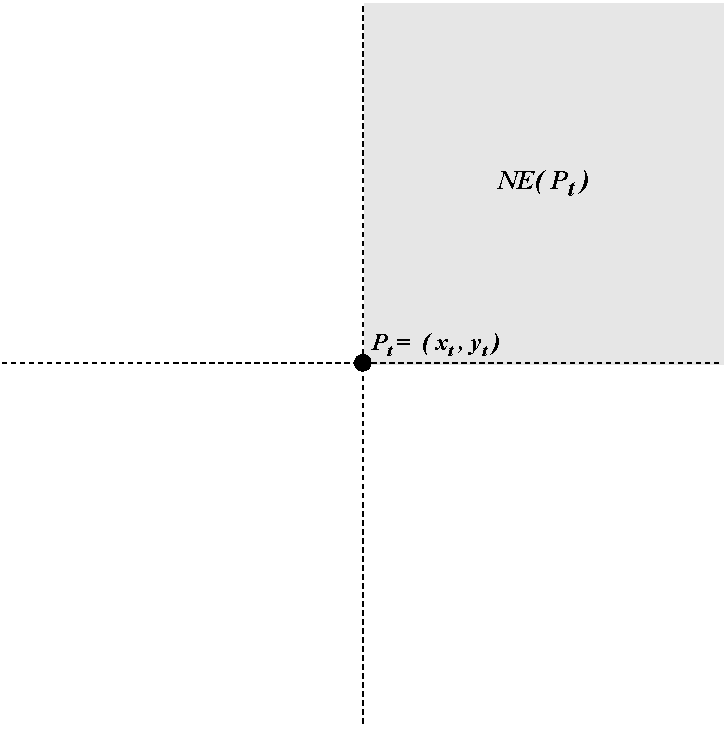
\includegraphics[scale=0.5]{img/NEP_t.pdf}
                \end{figure}
               $ NE(P_t) = \{(x_{i} , y_{i}) \in \mathbb{R}^2 | x_{i} > x_{t} \text{ และ } y_{i} > y_{t}\} $
            \end{center}
\end{frame}

\begin{frame}
\frametitle{การเเบ่งกั้นบริเวณรอบจุดเป้าหมาย}
\begin{center}
                \begin{figure}
                    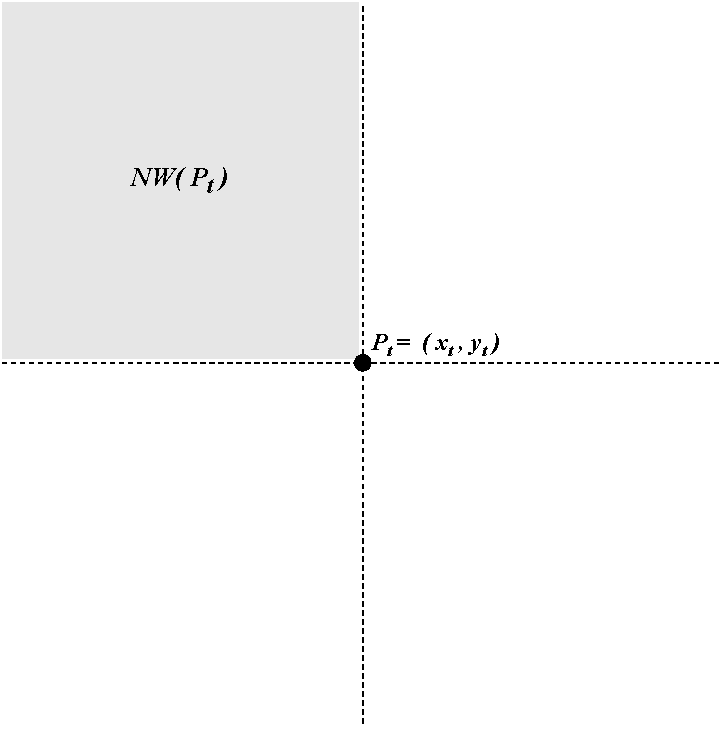
\includegraphics[scale=0.5]{img/NWP_t.pdf}
                \end{figure}
               $NW(P_t) = \{(x_{i} , y_{i}) \in \mathbb{R}^2 | x_{i} < x_{t} \text{ และ } y_{i} > y_{t}\}$
            \end{center}
\end{frame}

\begin{frame}
\frametitle{การเเบ่งกั้นบริเวณรอบจุดเป้าหมาย}
\begin{center}
                \begin{figure}
                    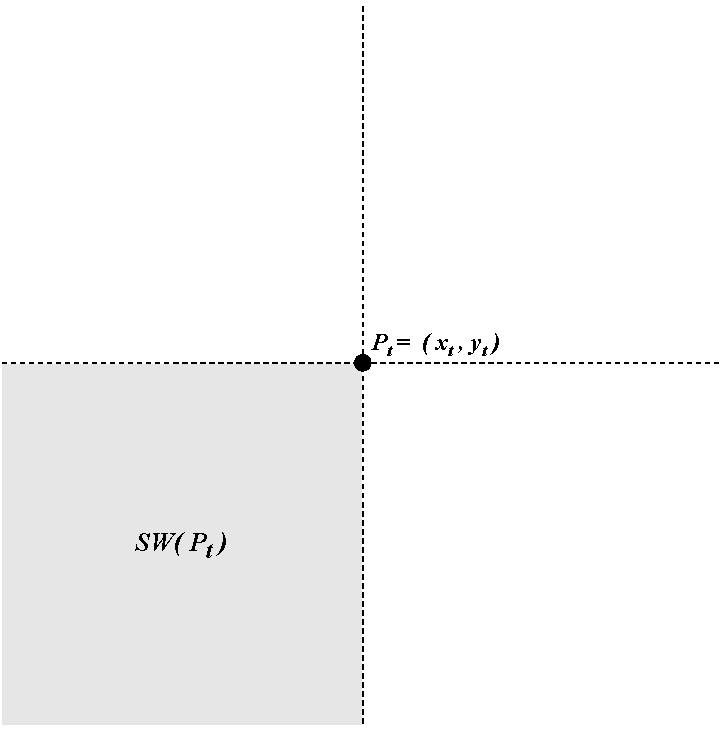
\includegraphics[scale=0.5]{img/SWP_t.pdf}
                \end{figure}
                $SW(P_t) = \{(x_{i} , y_{i}) \in \mathbb{R}^2 | x_{i} < x_{t} \text{ และ } y_{i} < y_{t}\} $
            \end{center}
\end{frame}

\begin{frame}
\frametitle{การเเบ่งกั้นบริเวณรอบจุดเป้าหมาย}
\begin{center}
        \begin{figure}
                    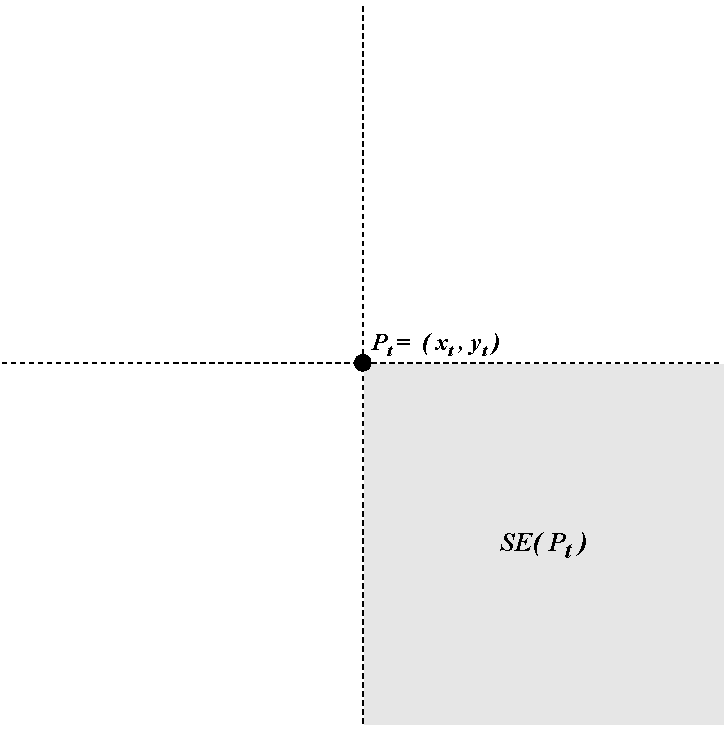
\includegraphics[scale=0.5]{img/SEP_t.pdf}
                \end{figure}
                $SE(P_t) = \{(x_{i} , y_{i}) \in \mathbb{R}^2 | x_{i} > x_{t} \text{ และ } y_{i} < y_{t}\}$
            \end{center}
\end{frame}

\begin{frame}
\frametitle{การเลือกจุดที่ล้อมรอบบริเวณเป้าหมาย}
    \begin{center}
        \begin{figure}
            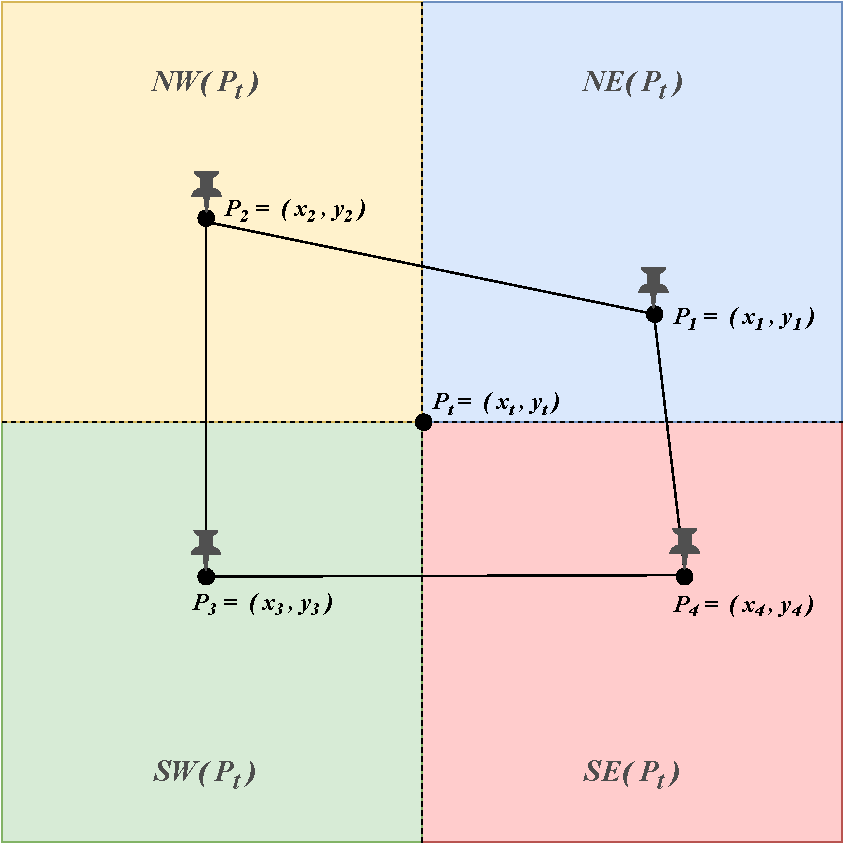
\includegraphics[scale=0.5]{img/selection.pdf}
        \end{figure}
    \end{center}
\end{frame}

\begin{frame}
    \frametitle{การพิจารณาเงื่อนไขจุดยอดของสี่เหลี่ยม }
\begin{theorem} 
	กำหนดให้ $P_i=(x_i,y_i) \in \mathbb{R}^2$ \text{และ}  $m_{ij} =\left(\dfrac{y_j-y_i}{x_j-x_i} \right)$ \text{ และ } $c_{ij} = y-m_{ij}x $ สำหรับ $i,j = 1,2,3,4$ และ $i \neq  j$ 
ถ้าเงื่อนไขต่อไปนี้เป็นจริง 
	\begin{enumerate}
\item \label{condition1} $x_{1}  \neq x_{2} \neq x_{3} \neq x_{4}$
\item \label{condition2} $y_3 - m_{12}x_3 + c_{12} \neq 0$
\item \label{condition3} $y_4 - m_{12}x_4 + c_{12} \neq 0$
\item \label{condition4} $y_4 - m_{23}x_4 + c_{23} \neq 0$
\item \label{condition5} $y_4 - m_{13}x_4 + c_{13} \neq 0$
\end{enumerate}
แล้ว $P_1,P_2,P_3$ และ $P_4$ เป็นจุดยอดของรูปสี่เหลี่ยม
\end{theorem}
\end{frame}

\begin{frame}{ตัวอย่าง}
    กำหนดให้  \[P_t = (1.75387,0.24043), \]
%$P_i=(x_i,y_i)$ และ $f(x_i,y_i)$ คือค่าดัชนีคุณภาพอากาศ ณ จุด $i$ โดยที่ $i=1,2,\ldots,10$
    \begin{center}
        \begin{tabular}{lccc} 
        \hline
       $P_i$ & ($x_i$,$y_i$) &  $f(x_i,y_i)$ \\
        \hline
        $P_1$ &$(1.75479,0.24063)$ &$74$\\
        $P_2$ &$(1.75516,0.24119)$ &$65$\\
        $P_3$ &$(1.75378,0.24084)$ &$63$\\
        $P_4$ &$(1.75296,0.24054)$ &$78$\\
        $P_5$ &$(1.75319,0.23996)$ &$78$\\
        $P_6$ &$(1.75292,0.23946)$ &$72$\\
        $P_7$ &$(1.75403,0.24010)$ &$89$\\
        $P_8$ &$(1.75396,0.23972)$ &$96$\\
        $P_9$ &$(1.75399,0.23909)$ &$87$\\
        $P_{10}$ &$(1.75570,0.24037)$ &$72$\\
        \hline
        \end{tabular}
    \end{center}
\end{frame}

% \begin{frame}
%     \frametitle{การแบ่งกั้นบริเวณรอบจุดเป้าหมาย}
%         \begin{definition}
%             กำหนดให้จุดเป้าหมาย คือ $P_t=(x_t,y_t) \in \mathbb{R}^2$ และกำหนดจุดที่ทราบค่าดัชนีคุณภาพอากาศที่อยู่รอบบริเวณจุดเป้าหมาย คือ $P_i=(x_i,y_i) \in \mathbb{R}^2$ สำหรับ $i=1,2,\ldots,n$ เรานิยามบริเวณรอบจุดเป้าหมาย $P_t$ ดังต่อไปนี้
%             \begin{align*}
%                 NE(P_t) &= \{(x_{i} , y_{i}) \in \mathbb{R}^2 | x_{i} > x_{t} \text{ และ } y_{i} > y_{t}\}\\
%                 NW(P_t) &= \{(x_{i} , y_{i}) \in \mathbb{R}^2 | x_{i} < x_{t} \text{ และ } y_{i} > y_{t}\}\\
%                 SW(P_t) &= \{(x_{i} , y_{i}) \in \mathbb{R}^2 | x_{i} < x_{t} \text{ และ } y_{i} < y_{t}\} \\
%                 SE(P_t) &= \{(x_{i} , y_{i}) \in \mathbb{R}^2 | x_{i} > x_{t} \text{ และ } y_{i} < y_{t}\}
%             \end{align*}
%             \end{definition}
%     \end{frame}
    
% \begin{frame}
%     \frametitle{การแบ่งกั้นบริเวณรอบจุดเป้าหมาย}
%     \begin{example}
%         \begin{center}
%             \begin{tabular}{lccc} 
%             \hline
%            $P_i$ & ($x_i$,$y_i$) &  บริเวณรอบจุดเป้าหมาย & $d(P_t,P_i)$\\
%             \hline
%             $P_1$ &$(1.75479291,0.24063575)$ &$NE(P_t)$  &$9.37439E-4$\\
%             $P_2$ &$(1.75516423,0.2411995)$ &$NE(P_t)$&$1.49599E-3$\\
%             $P_3$ &$(1.75378075,0.24084513)$ &$NW(P_t)$ &$4.18273E-4$\\
%             $P_4$ &$(1.75296025,0.24054795)$ &$NW(P_t)$&$9.22895E-4$\\
%             $P_5$ &$(1.75319981,0.23996681)$ &$SW(P_t)$&$8.24624E-4$\\
%             $P_6$ &$(1.75292431,0.23946067)$ &$SW(P_t)$&$1.36453E-3$\\
%             $P_7$ &$(1.75403828,0.24010061)$ &$SE(P_t)$&$3.74124E-4$\\
%             $P_8$ &$(1.75396042,0.23972831)$ &$SE(P_t)$&$7.146063E-4$\\
%             $P_9$ &$(1.75399636,0.23909994)$ &$SE(P_t)$&$1.34339E-3$\\
%             $P_{10}$ &$(1.75570923,0.24037401)$ &$SE(P_t)$&$1.83378E-3$\\
%             \hline
%             \end{tabular}
%         \end{center}
% \end{example}
% \end{frame}

\begin{frame}{ตัวอย่าง}
%    \frametitle{การแบ่งกั้นบริเวณรอบจุดเป้าหมาย}
        \begin{center}
            \begin{tabular}{lccc} 
            \hline
           $P_i$ & ($x_i$,$y_i$) &  บริเวณรอบจุดเป้าหมาย & $d(P_t,P_i)$\\
            \hline
            \cellcolor{orange!30}$P_1$ &\cellcolor{orange!30}$(1.75479,0.24063)$ &\cellcolor{orange!30}$NE(P_t)$  &\cellcolor{orange!30}$9.37E-4$\\
            $P_2$ &$(1.75516,0.24119)$ &$NE(P_t)$&$1.49E-3$\\
            \hline
            \cellcolor{orange!30}$P_3$ &\cellcolor{orange!30}$(1.75378,0.24084)$ &\cellcolor{orange!30}$NW(P_t)$ &\cellcolor{orange!30}$4.18E-4$\\
            $P_4$ &$(1.75296,0.24054)$ &$NW(P_t)$&$9.23E-4$\\
            \hline
            \cellcolor{orange!30}$P_5$ &\cellcolor{orange!30}$(1.75319,0.23996)$ &\cellcolor{orange!30}$SW(P_t)$&\cellcolor{orange!30}$8.25E-4$\\
            $P_6$ &$(1.75292,0.23946)$ &$SW(P_t)$&$1.36E-3$\\
            \hline
            \cellcolor{orange!30}$P_7$ &\cellcolor{orange!30}$(1.75403,0.24010)$ &\cellcolor{orange!30}$SE(P_t)$&\cellcolor{orange!30}$3.74E-4$\\
            $P_8$ &$(1.75396,0.23972)$ &$SE(P_t)$&$7.15E-4$\\
            $P_9$ &$(1.75399,0.23909)$ &$SE(P_t)$&$1.34E-3$\\
            $P_{10}$ &$(1.75570,0.24037)$ &$SE(P_t)$&$1.83E-3$\\
            \hline
            \end{tabular}
        \end{center}
\end{frame}

\begin{frame}{ตัวอย่าง}

พิจารณา $P_t = (x_t,y_t) =  (1.75387, 0.24043)$, $P_i = (x_i, y_i)$ โดยที่
\begin{columns}
\column{0.45\textwidth}
\begin{align*}
P_1 & = (1.75479, 0.24063) \in NE(P_t), \\ 
P_3 & = (1.75378, 0.24084) \in NW(P_t),\\
P_5 & = (1.75319, 0.23996) \in SW(P_t),\\
P_7 & = (1.75403, 0.24010)  \in SE(P_t), 
\end{align*}
\[m_{ij} = \dfrac{y_j-y_i}{x_j-x_i}, \]
\[c_{ij} = y_i - m_{ij}x_i,\]    
\column{0.45\textwidth} 
\begin{block}{}\
\textbf{จะได้ว่า} 
\begin{enumerate}
    \item $x_1 \neq x_3 \neq x_5 \neq x_7$
    \item $y_3 - m_{12}x_3 - c_{12} \neq 0$
    \item $y_4 - m_{12}x_4 - c_{12} \neq 0$
    \item $y_4 - m_{23}x_4 - c_{23} \neq 0$
    \item $y_4 - m_{13}x_4 - c_{13} \neq 0$
\end{enumerate}     
\end{block} 
\end{columns}


\end{frame}

%\begin{frame}
%    \frametitle{การตรวจสอบเงื่ิอนไขจุดยอดของสี่เหลี่ยม}
%        \textbf{เงื่อนไขข้อที่ $1$:} พิจารณา $1.75479 \neq 1.75378 \neq 1.75319 \neq 1.75403$
%
%ดังนั้น  $x_1 \neq x_3 \neq x_5 \neq x_7$
%
%\vspace{1cm}
%\textbf{เงื่อนไขข้อที่ $2$:} พิจารณา
%\begin{align*} 
%m_{ij} &=\left(\dfrac{y_j-y_i}{x_j-x_i} \right)\\
%m_{13} &=\left(\dfrac{y_3-y_1}{x_3-x_1} \right)\\
%       &=\left(\dfrac{0.24084-0.24063}{1.75378-1.75479} \right)\\
%       &=-0.20686
%\end{align*}
%\end{frame}
%
%\begin{frame}
%    \frametitle{การตรวจสอบเงื่ิอนไขจุดยอดของสี่เหลี่ยม}
%\begin{align*} 
%    c_{ij} &= y_1-m_{ij}x_1\\ 
%    c_{13} &= y_1-m_{13}x_1\\
%           &= 0.24043798-(-0.20683489)(1.75387657)\\
%           &= 0.60320085
%\end{align*}
%\begin{align*} 
%    y_5 - m_{13}x_5 + c_{13} & = 0.23996681 -(-0.20683489)(1.75319981) + 0.60320085\\
%   & = 1.20579055
%\end{align*}
%เนื่องจาก $1.20579055 \neq 0$
%
%ดังนั้น $y_5 - m_{13}x_5 + c_{13} \neq 0 $
%\end{frame}
%
%\begin{frame}
%    \frametitle{การตรวจสอบเงื่ิอนไขจุดยอดของสี่เหลี่ยม}
%    ในทำนองเดียวกันเงื่อนไขข้อที่ $3,4$ และ $5$ ได้ผลลัพธ์ดังนี้
%% \begin{align*}
%%     1.20609777 &\neq 0\\
%%     -4.8236405 &\neq 0\\
%%     -1.04282178 &\neq 0
%%     \end{align*}
%\begin{align*}
%    y_7 - m_{13}x_7 + c_{13} &\neq 0\\
%    y_7 - m_{57}x_7 + c_{57} &\neq 0\\
%    y_7 - m_{17}x_7 + c_{17} &\neq 0
%    \end{align*}
%
%    \vspace{0.5cm}
%    ดังนั้น เราสามารถสร้างสี่เหลี่ยมที่มีจุด $P_1,P_3,P_5$ และ $P_7$ เป็นจุดยอดได้
%\end{frame}

\begin{frame}{ตัวอย่าง}
        \begin{columns}
            \begin{column}{0.6\textwidth}
\begin{align*}
f(P_1) & = f(x_1,y_1) = f(1.75479, 0.24063) = 74, \\ 
f(P_3) & = f(x_3,y_3) = (1.75378, 0.24084) = 63,\\
f(P_5) & = f(x_5,y_5) = f(1.75319, 0.23996) = 78,\\
f(P_7) & = f(x_7,y_7) = f(1.75403, 0.24010) = 89, 
\end{align*}
จะได้ว่า
%\vspace{-7mm}
            \begin{block}{}
            \vspace{-3mm}
              \begin{align*}
                 f(P_t) & = f(x_t,y_t) \\
                        & = f(1.75387, 0.24043)\\
                        & = a+bx_t+cy_t+dx_ty_t \\
                        & \approx 75.83
              \end{align*}  
            \end{block}

            \end{column}
            \begin{column}{0.35\textwidth} 

{\color{orange!90!black}%
เมื่อ $a,b,c$ และ $d$ คือผลเฉลยของสมการ $AX = B$  โดยที่              
            \[
               A
               =\begin{bmatrix}
               1 & x_1 & y_1 & x_1y_1\\
               1 & x_3 & y_3 & x_3y_3\\
               1 & x_5 & y_5 & x_5y_5\\
               1 & x_7 & y_7 & x_7y_7\\
               \end{bmatrix},
        \]
        \[
               X = \begin{bmatrix}
                  a \\ b \\ c \\ d
               \end{bmatrix}
               ,
               B
               =\begin{bmatrix}
                  f(x_1,y_1) \\
                  f(x_3,y_3) \\
                  f(x_5,y_5) \\
                  f(x_7,y_7)
               \end{bmatrix}
        \]
}
            \end{column}

            \end{columns}    
\end{frame}

%\begin{frame}
%    \frametitle{การประมาณค่าเชิงเส้นคู่แบบทางเลือก}
%    \begin{align*}
%        P_t &= (x_t,y_t)=(1.75387,0.24043) \\
%        P_1& =(x_1,y_1)=(1.75479,0.24063) \text{ และ } f(P_1) = 74 \\
%        P_3&=(x_3,y_3)=(1.75378,0.24084) \text{ และ } f(P_3) = 63\\ 
%        P_5&=(x_5,y_5)=(1.75319,0.23996) \text{ และ } f(P_5) = 78\\
%        P_7&=(x_7,y_7)=(1.75403,0.24010) \text{ และ } f(P_7) = 89
%     \end{align*}
%    \begin{equation}\label{alternative-bilinear-interpolation7}
%        f(x_t,y_t)=a+bx_t+cy_t+dx_ty_t
%   \end{equation}
%   
%   เมื่อ $a,b,c$ และ $d$ คือผลเฉลยของสมการ 
%   
%   \begin{equation}\label{linear-system-equation}
%      AX = B  
%   \end{equation}
%   
%   โดยที่
%   
%   \begin{equation*}
%   A
%   =\begin{bmatrix}
%   1 & x_1 & y_1 & x_1y_1\\
%   1 & x_3 & y_3 & x_3y_3\\
%   1 & x_5 & y_5 & x_5y_5\\
%   1 & x_7 & y_7 & x_7y_7\\
%   \end{bmatrix}
%   ,
%   \quad
%   X
%   =\begin{bmatrix}
%      a\\
%      b\\
%      c\\	
%      d
%   \end{bmatrix}
%   ,
%   \quad
%   B
%   =\begin{bmatrix}
%      f(x_1,y_1)\\
%      f(x_3,y_3)\\
%      f(x_5,y_5)\\
%      f(x_7,y_7)
%   \end{bmatrix}
%   \end{equation*}
%\end{frame}
%
%\begin{frame}
%    \frametitle{การประมาณค่าเชิงเส้นคู่แบบทางเลือก}
%   จากสมการ \eqref{linear-system-equation} จะได้ผลเฉลย $a,b,c$ และ $d$ ดังนี้ 
%   \begin{align*}
%    a&=-30437137.8977641\\
%    b&=17339545.86913783\\
%    c&=126855602.2007634
%   \end{align*}
%และ 
%\begin{equation*}
%d=-72267353.90469953
%\end{equation*}
%ตามลำดับ
%\vspace{0.5cm}
%
%\hspace{0.5cm} นำ $a,b,c$ และ $d$ แทนลงในสมการ \eqref{alternative-bilinear-interpolation7} จะได้ว่า $f(x_t,y_t) \approx 75.83$
%
%ดังนั้น ณ จุดเป้าหมาย  $P_t$ มีค่าประมาณของดัชนีคุณภาพอากาศเท่ากับ $75.83$ 
%\end{frame}

\begin{frame}
    \frametitle{ค่าคลาดเคลื่อน}

    \begin{tikzpicture}[overlay, remember picture]
        \node at (7,-2.8) {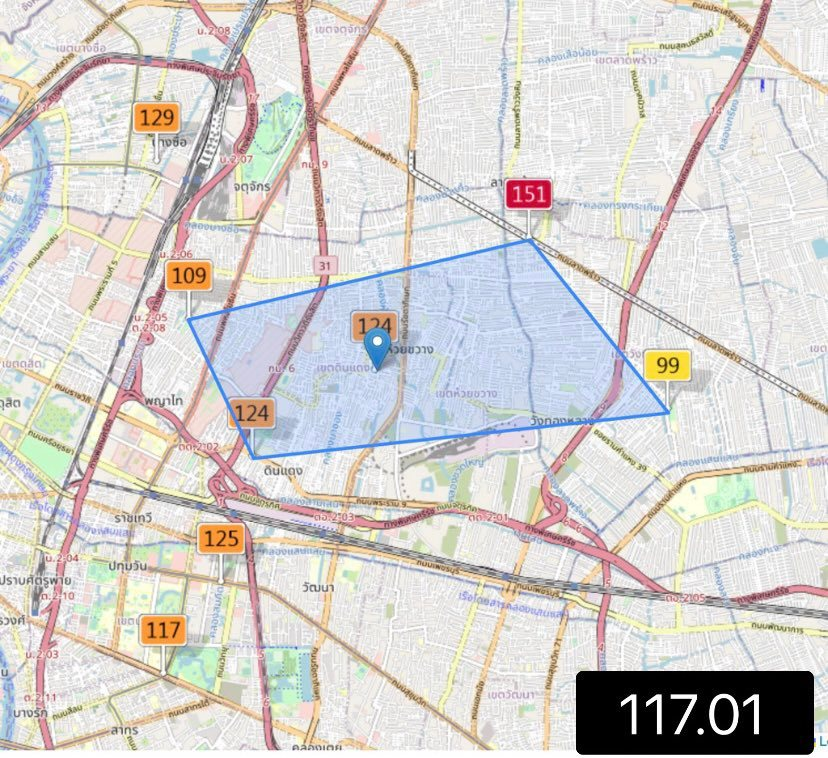
\includegraphics[width=1.25\textwidth]{img/error-test.jpg}};
        \node[fill=white, rounded corners=0.1cm] (p) at (9,0) {\Huge \texttt{117}};
        \draw[->, white, line width=1.5mm] (p) -- (6.1,-0.8);
    \end{tikzpicture}    
    \end{frame}

\begin{frame}
    \frametitle{ค่าความคลาดเคลื่อน}
\begin{center}
    \begin{tabular}{lcc} 
        \hline
        $P_i$ & ละติจูด & ลองจิจูด \\
        \hline
        1 & 13.90451806 & 100.5277991   \\
        2 & 13.77523348 & 100.5695343  \\
        3 & 13.72971342 & 100.5365753 \\
        4 & 13.76206192 & 100.5506516  \\
        5 & 13.77640054 & 100.5697083\\
        6 & 13.05272355 & 101.1030755\\
        7 & 13.72954666 & 100.5363191 \\
        8 & 13.72988017 & 100.5364923 \\
        9 & 18.25021998 & 99.76271963\\
        10 & 17.16178591 & 104.1341291 \\
        \hline
        \end{tabular}
    \end{center}
\end{frame}

\begin{frame}
    \frametitle{ค่าความคลาดเคลื่อน}
        \begin{center}
        \begin{tabular}{lccccc} 
        \hline
        $P_i$ & ค่าจริง &ค่าประมาณ &  ค่าคาดเคลื่อน & ร้อยละค่าคลาดเคลื่อน\\
        \hline
        1 & 152 & 139.46   &12.54 &8.25\% \\
        2 &124 & 117.01   &6.99  &5.64\% \\
        3  &127   & 137.5   &10.5  &8.27\% \\
        4  &122  & 108.35   &13.65 &11.19\% \\
        5 &129 & 104.56   &24.44 &18.95\% \\
        6  &127  & 121.15   &5.85  &4.61\% \\
        7&152 & 131.48   &20.52 &13.50\% \\
        8  &152 & 138.13   &13.87 &9.13\% \\
        9 &89 & 104.83   &15.83 &17.79\% \\
        10 &97 & 150.97   &53.97 &55.64\% \\
        \hline
        \end{tabular}
    \end{center}
\end{frame}

\begin{frame}
    \frametitle{Web application}
        \begin{center}
            \begin{figure}
                \centering
                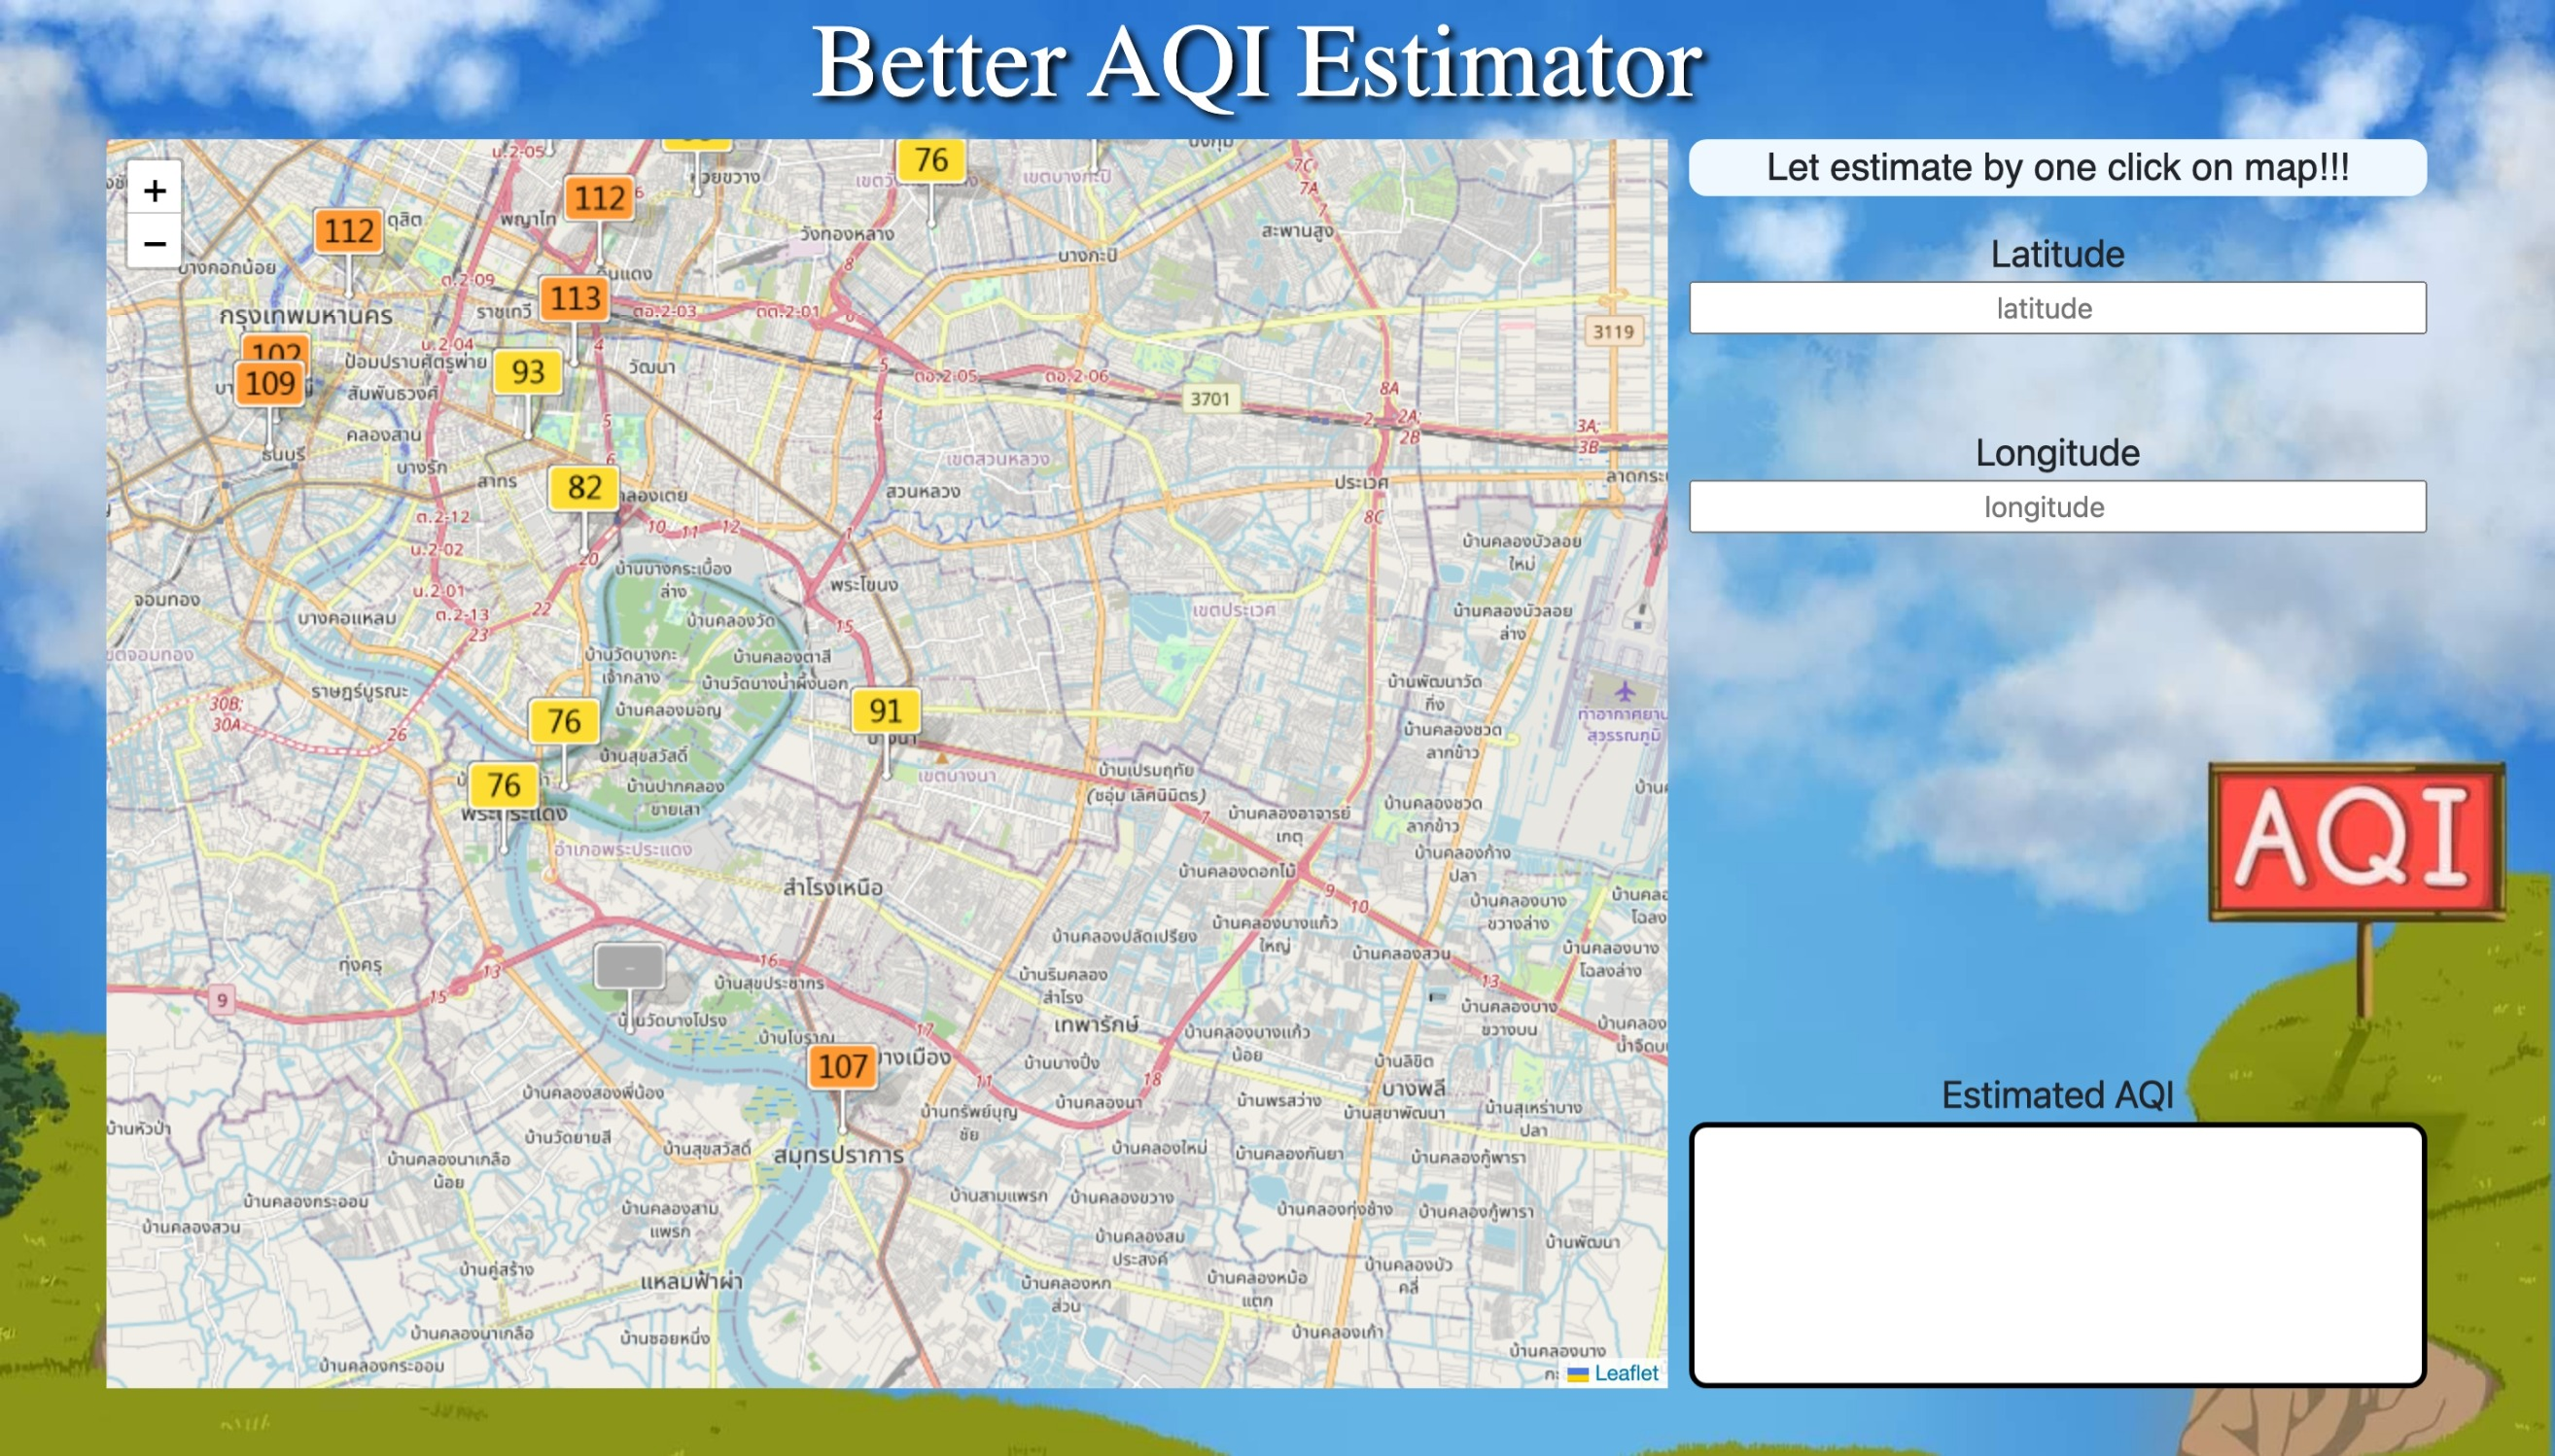
\includegraphics[width=\textwidth]{img/web-app.jpeg}
            \end{figure}
        \end{center}
    \end{frame}

\begin{frame}
\frametitle{Tech Stack}
    \begin{center}
        \begin{figure}
            \centering
            
\includegraphics[width=\textwidth]{img/tech-stack.pdf}
        \end{figure}
    \end{center}
\end{frame}

\end{document}